\documentclass{article}

\usepackage{amsmath}
\usepackage{amssymb}
\usepackage{enumerate}
\usepackage[spanish]{babel}
\usepackage{cancel}
\usepackage{caption}
\usepackage[margin=1.5in]{geometry}
\usepackage{graphicx}
\usepackage[utf8]{inputenc}
\usepackage{tcolorbox}
\usepackage{esint}
\usepackage{hyperref}
\hypersetup{
    colorlinks,
    citecolor=black,
    filecolor=black,
    linkcolor=black,
    urlcolor=black,
}

\renewcommand{\Bbb}{\mathbb}

\tcbuselibrary{theorems}

\title{Ejercicios de Análisis Matemático II A (63.01) \\ Cátedra Acero \\ 1° C 2004}
\author{Darío Eduardo Ramos}

\begin{document}
\maketitle

\tableofcontents{}
\newpage

\section{Geometría del plano y el espacio}

\hrule
\vspace{10 pt}

\textbf{1. Hallar en cada caso la ecuación implícita de un plano que satisfaga las condiciones dadas. Analizar si esas condiciones determinan el plano unívocamente.} 

\begin{enumerate}[(a)]
\bfseries
\item pasa por $(1, 1, 0)$, $(0, 2, 1)$ y $(3, 2, -1)$;

\item pasa por $(2, 0, 1)$ y es perpendicular a la recta que pasa por $(1, 1, 0)$ y $(4, -1, -2)$;

\item contiene a la intersección de los planos de ecuaciones $x + y - 2z = 0$ y $2x - y + z = 2$;

\item es perpendicular al plano de ecuación $2x + 3y + 4z = 5$ y contiene a la recta de ecuaciones $x + y = 2$, $y - z = 3$.
\end{enumerate}
\hrule

\begin{enumerate}[a)]

\item En $\Bbb R^n$, $n$ puntos distintos determinan unívocamente un plano $\Leftrightarrow$ no son colineales. Concretamente, no están sobre la misma recta; esto equivale a exigir que los vectores que los unen no son paralelos. En este caso:

\begin{subequations}
\begin{align}
& P = (1, 1, 0) \wedge Q = (0, 2, 1) \wedge R = (3, 2, -1) \\
& \overline{PQ} = Q - P = (0-1, 2-1, 1-0) = (-1, 1, 1) \\
& \overline{QR} = R - Q = (3-0, 2-2, -1-1) = (3, 0, -2)
\end{align}
\end{subequations}

Estos vectores no son múltiplos entre sí, y por ende no son colineales, y el plano que determinan es único. Para calcular la expresión implícita de dicho plano, vale decir:

\begin{subequations}
\begin{align}
a (x-x_0) + b (y-y_0) + c (z-z_0) = 0 \\
a x + b y + c z + d = 0, d = -a x_0 -b y_0 -c z_0
\end{align}
\end{subequations}

Nótese que la ecuación del plano es un producto escalar igualado a cero (con una constante de ajuste). Ergo, el vector $(a,b,c)$ es ortogonal al plano. Por lo tanto, puede obtenerse haciendo el producto vectorial entre dos vectores no colineales pertenecientes al plano, como lo son $\overline{PQ}$ y $\overline{QR}$:

\begin{subequations}
\begin{align}
(a,b,c) &= \overline{PQ} \times \overline{QR} = \det \begin{vmatrix}
\hat{i} & \hat{j} & \hat{k} \\
-1 & 1 & 1 \\
3 & 0 & -2
\end{vmatrix} = \hat{i} \begin{vmatrix}1 & 1 \\ 0 & -2\end{vmatrix} - \hat{j} \begin{vmatrix}-1 & 1 \\ 3 & -2\end{vmatrix} + \hat{k} \begin{vmatrix}-1 & 1 \\ 3 & 0\end{vmatrix} \\
& = \hat{i} (-2-0) -\hat{j} (2-3) +\hat{k} (0-3) = (-2, 1, -3)
\end{align}
\end{subequations}

Obtenido el vector normal $(a,b,c)$, reemplazando cualquier vector perteneciente al plano como $(x_0, y_0, z_0)$, se obtiene la ecuación implícita buscada. Por ejemplo, con $(x_0, y_0, z_0) = P = (1, 1, 0)$:

\begin{equation}
-2 (x-1) + 1 (y-1) - 3 (z-0) = 0 \Rightarrow -2x +2 +y -1 -3z = 0 
\end{equation}

\begin{equation}
\tcboxmath[colback=orange!25!white,colframe=orange, title=Plano único]
{ -2x +y -3z + 1 = 0 }
\end{equation}

\item Dadas una recta, hay infinitos planos perpendiculares a ella. Sin embargo, especificando un punto del plano, incluso si es sobre la recta, determina unívocamente el plano. Por lo tanto, en este caso también resulta único el plano.

Si la recta es perpendicular al plano, su vector dirección sirve como vector normal del plano, o sea $(a,b,c)$ en la ecuación implícita del plano. Para obtener el vector dirección de una recta, basta con restar dos puntos de la misma:

\begin{equation}
(a, b, c) = (1, 1, 0) - (4, -1, -2) = (-3, 2, 2)
\end{equation}

Y dado que también se tiene un punto del plano, reemplazándolo como $(x_0, y_0, z_0)$ se obtiene de forma directa la ecuación del plano:

\begin{subequations}
\begin{align}
& a (x-x_0) + b (y-y_0) + c(z-z_0) = 0 \\
& -3 (x-2) + 2 (y-0) + 2 (z-1) = 0 \Rightarrow -3x + 2y + 2z +6-2 = 0
\end{align}
\end{subequations}

\begin{equation}
\tcboxmath[colback=orange!25!white,colframe=orange, title=Plano único]
{ -3x + 2y +2z + 4 = 0 }
\end{equation}

\item La intersección de dos planos puede ser vacía, una recta o un plano (si son el mismo plano). Ergo, la única forma de que la intersección de dos planos determine unívocamente un plano es que los dos planos sean el mismo. En todo caso, resolver el sistema de ecuaciones dará la respuesta.

\begin{subequations}
\begin{align}
\left\{
\begin{array}{ll}
x + y -2z = 0 \\
2x -y + z = 2
\end{array}
\right. \overset{R_2 \leftarrow -2R_1 + R_2}{\Longrightarrow}
\left\{
\begin{array}{ll}
x & + y -2z = 0 \\
  & - 3y + 5z = 2
\end{array}
\right.
\end{align}
\end{subequations}

Hay dos ecuaciones l.i. entre sí, y 3 incógnitas. Por lo tanto, hay un grado de libertad y la solución es una recta. La expresión paramétrica de la misma puede hallarse, por ejemplo, despejando $z$ en función de $y$ en $R_2$ y reemplazando en $R_1$ para hallar $x$ en función de $y$:

\begin{subequations}
\begin{align}
& R_2: 5z = 2 + 3y \Rightarrow z = \frac{2}{5} + \frac{3}{5} y \\
& R_1: x + y - 2 \left( \frac{2}{5} + \frac{3}{5} y \right) = 0 \Rightarrow x + y -\frac{4}{5} - \frac{6}{5} y = 0 \Rightarrow x = \frac{4}{5} + \frac{1}{5} y
\end{align}
\end{subequations}

Pensando en $y$ como el parámetro $\lambda$, la intersección buscada es la recta $R$:

\begin{subequations}
\begin{align}
& R: \left( \frac{4}{5} + \frac{1}{5} \lambda, \lambda, \frac{2}{5} + \frac{3}{5} \lambda \right) \\
& R: \left(\frac{1}{5}, 1, \frac{3}{5} \right) \lambda + \left(\frac{4}{5}, 0, \frac{2}{5} \right) \\
& R: (1, 5, 3) t + (4, 0, 2)
\end{align}
\end{subequations}

Por la recta $R$, pasan infinitos planos. Con elegir un punto fuera de la recta, alcanza para determinar uno cualquiera. Con que tenga un valor distinto de $5$ en la componente $y$ es suficiente, por lo tanto se elige $(0, 1, 0)$. Tomando ese punto y dos puntos de la recta, los de $t=0$ y $t=1$, se tienen 3 puntos para determinar un plano de todos los posibles:

\begin{subequations}
\begin{align}
& P = (0, 1, 0) \wedge Q = (4, 0, 2) \wedge R = (5, 5, 5) \\
& \overline{PQ} = Q - P = (4-0, 0-1, 2-0) = (4, -1, 2) \\
& \overline{QR} = R - Q = (5-4, 5-0, 5-2) = (1, 5, 3) \\
& (a, b, c) = \overline{PQ} \times \overline{QR} = \begin{vmatrix}
\hat{i} & \hat{j} & \hat{k} \\
4 & -1 & 2 \\
1 & 5 & 3
\end{vmatrix} = \hat{i} \begin{vmatrix}
-1 & 2 \\
5 & 3
\end{vmatrix} -\hat{j} \begin{vmatrix}
4 & 2 \\
1 & 3
\end{vmatrix} +\hat{k} \begin{vmatrix}
4 & -1 \\
1 & 5
\end{vmatrix} = \\
& (a, b, c) = (-3-10, -(12-2), 20-(-1)1) = (-13, -10, 21) \\
& -13 (x-0) -10 (y-1) +21 (z-0) = 0
\end{align}
\end{subequations}

\begin{equation}
\tcboxmath[colback=orange!25!white,colframe=orange, title=Un plano de infinitos posibles]
{ -13x - 10y + 21z + 10 = 0 }
\end{equation}

\item Sean:

\begin{subequations}
\begin{align}
& \Pi: 2x + 3y + 4z = 5 \text{ el plano dato} \\
& R: \left\{ \begin{array}{ll}
x + y = 2 \\
y - z = 3
\end{array} \right. \text{ la recta que debe estar contenida en } \Phi \\
& \Phi: \text{ El plano a determinar, perpendicular a } \Pi \text{, contiene a R}
\end{align}
\end{subequations}

Para que $\Phi$ contenga a $R$ y a la vez sea perpendicular a $\Pi$, es necesario que $R$ sea paralela a la normal del plano. Para determinar el vector dirección de $R$, se la pasa a su forma paramétrica:

\begin{subequations}
\begin{align}
& R_1: x = 2 - y \\
& R_2: -z = 3 - y \Rightarrow z = -3 + y \\
& R: (2-\lambda, \lambda, -3+\lambda) = (-1, 1, 1) \lambda + (2, 0, -3) \\
& \overline{v_R} = R(t=0) - R(t=1) = (2, 0, -3) - (1, 1, -2) = (1, -1, -1)
\end{align}
\end{subequations}

Dado que $R$ no es paralela a la normal de $\Pi$ (porque $(2, 3, 4)$ no es paralelo a $(1, -1, -1)$), no existe un plano perpendicular a $\Pi$ que contenga por completo a $R$. 

\end{enumerate}

\hrule
\vspace{10 pt}
\textbf{2. Hallar en cada caso las ecuaciones implícitas de una recta que satisfaga las condiciones dadas. Analizar si esas condiciones determinan la recta unívocamente.} 

\begin{enumerate}[(a)]
\bfseries
\item pasa por el origen y es paralela a la recta de ecuaciones $x + 2y -z = 2, 2x - y + 4z = 5$

\item pasa por $(1, 2, -1)$ y forma con los tres semiejes positivos ángulos iguales entre sí.

\item está determinada como intersección de los planos de ecuaciones $y-x = 0$ y $z = 4 - x - y$
\end{enumerate}
\hrule

\begin{enumerate}[(a)]

\item Sean:

\begin{subequations}
\begin{align}
& R_1: \left\{ \begin{array}{ll}
x + 2y - z = 2 \\
2x - y + 4z = 5
\end{array} \right. \\
& R_2: \text{Recta a determinar. Pasa por } (0, 0, 0) \text{ y es paralela a } R_1
\end{align}
\end{subequations}

Respecto a la unicidad, $R_2$ está especificada por un punto y un vector dirección (paralelo al de $R_1$), por lo cual está garantizada su unicidad. Como primer paso, paso $R_1$ a forma paramétrica para obtener su vector dirección:

\begin{subequations}
\begin{align}
& \left\{ \begin{array}{l}
x + 2y -z = 2 \\
2x - y + 4z =5
\end{array} \right. \overset{F_2 \leftarrow -2F_1 + F_2}{\sim} \left\{ \begin{array}{rr}
x + 2y - z = 2 \\
-5y + 6z = 1
\end{array} \right. \\
& \text{Despejando } z \text{ en } F_2: 6z = 1 + 5y \Rightarrow z = \frac{1}{6} + \frac{5}{6} y \\
& \text{Reemplazando en } F_1: x + 2y - \frac{1}{6} -\frac{5}{6} y = 2 \Rightarrow x = \frac{13}{6} - \frac{7}{6} y \\
& R_1 : \left(\frac{13}{6} - \frac{7}{6} \lambda, \lambda, \frac{1}{6} + \frac{5}{6} \lambda \right) = \left(-\frac{7}{6}, 1, \frac{5}{6}\right) \lambda + \left(\frac{13}{6}, 0, \frac{1}{6}\right) \\
& R_1: (-7, 6, 5) \lambda + (13, 0, 1)
\end{align}
\end{subequations}

Como $R_2$ es paralela a $R_1$, tienen el mismo vector dirección. Y como $R_2$ pasa por el origen, resulta $R_2: (-7, 6, 5) \lambda $. Pasando a implícitas:

\begin{equation}
\frac{x}{-7} = \frac{y}{6} = \frac{z}{5} \Rightarrow R_2: \left\{ \begin{array}{ll}
6x = -7y \\
5y = 6z
\end{array} \right.
\end{equation}

\begin{equation}
\tcboxmath[colback=orange!25!white,colframe=orange, title=Recta única]
{ \left\{ \begin{array}{llr}
6x + &7y &= 0 \\
&5y - 6z &= 0
\end{array} \right. }
\end{equation}

\item Se está definiendo un punto, ¿pero cuántas direcciones posibles hay? La forma más sencilla de verlo es primero trabajando en el plano $xy$, y $z$ deberá tener el mismo ángulo. En el plano $xy$, visualizando la proyección de la recta, hay dos posibilidades, como se observa en la figura \ref{fig:1-2-b}.

\begin{figure}[ht]
\caption{Rectas con igual ángulo respecto a semiejes positivos}
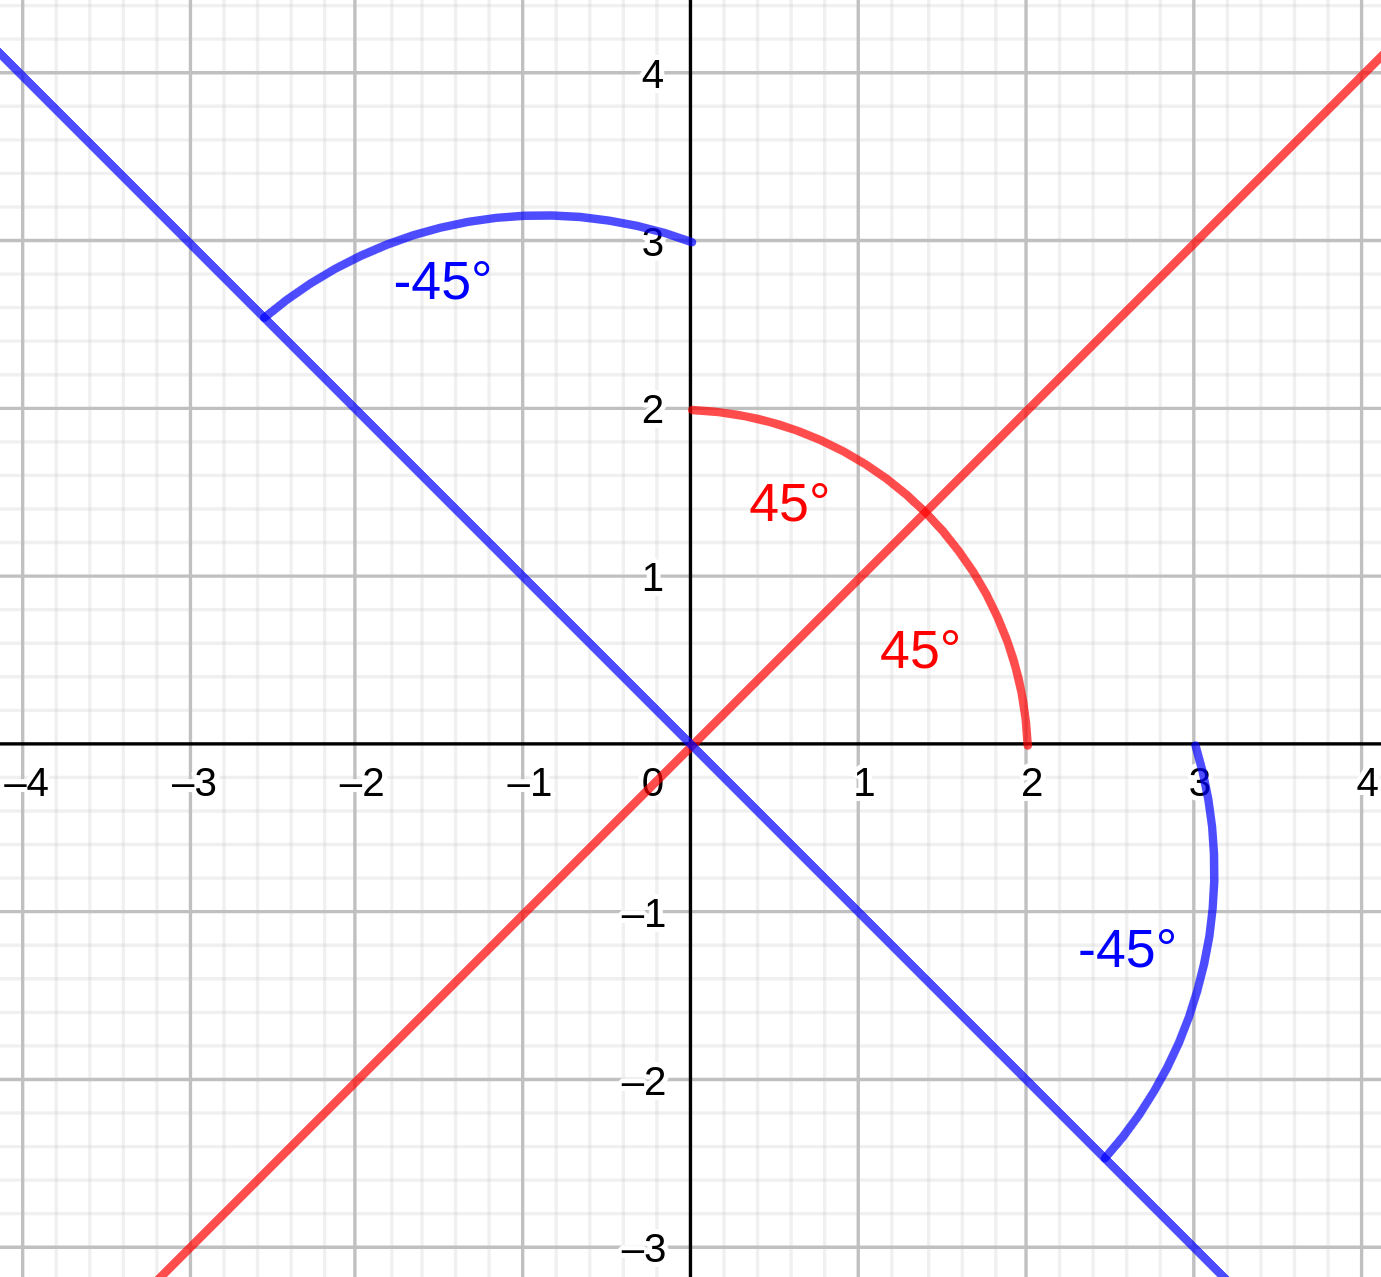
\includegraphics[scale=1]{img/ejercicios/1/2-b.png} 
\centering
\label{fig:1-2-b}
\end{figure}

Dado que cada uno de estos dos casos fija el valor del ángulo respecto al semieje positivo $z$, hay dos direcciones posible para la recta: $(1, 1, 1)$ y $(1, -1, -1)$. Eligiendo arbitrariamente la primera, con el punto dado resulta:

\begin{equation}
R: (1, 1, 1) \lambda + (1, 2, -1) 
\end{equation}

Pasando a ecuaciones implícitas:

\begin{equation}
\frac{x-1}{1} = \frac{y-2}{1} = \frac{z+1}{1} \Rightarrow \left\{ \begin{array}{ll}
x-1 = y - 2 \\
y-2 = z + 1
\end{array} \right.
\end{equation}

\begin{equation}
\tcboxmath[colback=orange!25!white,colframe=orange, title=Una de dos rectas posibles]
{ R: \left\{ \begin{array}{llr}
x - &y &= 0 \\
&y - z - 3 &= 0
\end{array} \right. }
\end{equation}

\item Las ecuaciones implícitas de una recta son, por definición, la intersección entre dos planos. Sólo restaría acomodar los términos y verificar si la intersección es una recta:

\begin{equation}
\left\{ \begin{array}{ll}
y-x = 0 \\
z = 4-x-y
\end{array} \right. \sim \left\{ \begin{array}{llr}
-x &+ y &= 0 \\
x &+ y + z -4 &= 0
\end{array} \right.
\end{equation}

No hace falta ninguna transformación para ver que las dos ecuaciones son l.i., y por ende determinan una única recta.

\begin{equation}
\tcboxmath[colback=orange!25!white,colframe=orange, title=Recta única]
{ \left\{ \begin{array}{llr}
-x &+ y &= 0 \\
x &+ y + z -4 &= 0
\end{array} \right. }
\end{equation}

\end{enumerate}

\hrule
\vspace{10 pt}
\textbf{3. En los siguientes casos, hallar $k$ de manera que exista más de un plano que pase por $v_1$, $v_2$ y $v_3$. Analizar una condición aplicable en general.} 

\begin{enumerate}[(a)]
\bfseries
\item $v_1 = (1, 0, 0)$, $v_2=(0, 1, 0)$, $v_3 = (2, -1, k)$;

\item $v_1 = (1, 1, 0)$, $v_2=(1, -1, 1)$, $v_3 = (1, -3, k)$
\end{enumerate}
\hrule

\begin{enumerate}[(a)]

\item Para que 3 puntos determinen más de un plano, deben ser colineales: sus vectores diferencia deben ser paralelos.

\begin{subequations}
\begin{align}
& \overline{v_{12}} = v_2 - v_1 = (-1, 1, 0) \\
& \overline{v_{23}} = v_3 - v_2 = (2, -2, k) \\
& \overline{v_{12}} \parallel \overline{v_{23}} \Leftrightarrow \overline{v_{12}} = \alpha \overline{v_{23}} \Leftrightarrow \left\{ \begin{array}{ll}
-1 = \alpha 2 \\
1 = \alpha (-2) \\
0 = \alpha k
\end{array} \right. \Leftrightarrow \left\{ \begin{array}{ll}
\alpha = -\frac{1}{2} \\
\alpha = -\frac{1}{2} \\
0 = \alpha k
\end{array} \right.
\end{align}
\end{subequations}

\begin{equation}
\tcboxmath[colback=orange!25!white,colframe=orange]
{ k = 0 }
\end{equation}

\item Aplicando el mismo método:

\begin{subequations}
\begin{align}
& \overline{v_{12}} = v_2 - v_1 = (0, -2, 1) \\
& \overline{v_{23}} = v_3 - v_2 = (0, -2, k-1) \\
& \overline{v_{12}} \parallel \overline{v_{23}} \Leftrightarrow \overline{v_{12}} = \alpha \overline{v_{23}} \Leftrightarrow \left\{ \begin{array}{ll}
0 = \alpha 0 \\
-2 = \alpha (-2) \\
1 = \alpha (k-1)
\end{array} \right. \Leftrightarrow \left\{ \begin{array}{ll}
0 = 0 \\
\alpha = 1 \\
1 = \alpha (k-1)
\end{array} \right.
\end{align}
\end{subequations}

\begin{equation}
\tcboxmath[colback=orange!25!white,colframe=orange]
{ k = 2 }
\end{equation}

Para analizar una condición general, se plantean $v_1$, $v_2$ y $v_3$ genéricos:

\begin{subequations}
\begin{align}
& v_1 = (v_{1x}, v_{1y}, v_{1z}), v_2 = (v_{2x}, v_{2y}, v_{2z}), v_3 = (v_{3x}, v_{3y}, v_{3z}) \\
& \overline{v_{12}} = v_2 - v_1 = (v_{2x} - v_{1x}, v_{2y} - v_{1y}, v_{2z} - v_{1z}) \\
& \overline{v_{23}} = v_3 - v_2 = (v_{3x} - v_{2x}, v_{3y} - v_{2y}, v_{3z} - v_{2z}) \\
& \overline{v_{12}} \parallel \overline{v_{23}} \Leftrightarrow \overline{v_{12}} = \alpha \overline{v_{23}} \Leftrightarrow \left\{ \begin{array}{ll}
v_{2x} - v_{1x} = \alpha (v_{3x} - v_{2x}) \\
v_{2y} - v_{1y} = \alpha (v_{3y} - v_{2y}) \\
v_{2z} - v_{1z} = \alpha (v_{3z} - v_{2z})
\end{array} \right.
\end{align}
\end{subequations}

Despejando $\alpha$ en las 3 ecuaciones e igualando, resulta la condición general buscada:

\begin{equation}
\tcboxmath[colback=orange!25!white,colframe=orange]
{ \frac{v_{2x} - v_{1x}}{v_{3x} - v_{2x}} = \frac{v_{2y} - v_{1y}}{v_{3y} - v_{2y}} = \frac{v_{2z} - v_{1z}}{v_{3z} - v_{2z}} }
\end{equation}

\end{enumerate}

\end{document}